% Contributors: Luis Lopez, Robby Costales, Daniel Jaroslawicz, Colin Brown
\section{GANs}

\subsection{Game Formulation}
The central idea behind Generative Adversarial Networks, as the name would suggest, is that if a generative model is supposed to create realistic examples of a given input, then its output shouldn't be easily differentiable from examples of the original input. With this in mind, Goodfellow et al. \cite{goodfellow2014generative} proposed an adversarial training framework under which a generative model would be trained jointly with an adversary, with the generative model learning to create output like its input just as the adversary learns to discriminate real input from the fake, generated examples from the generative model.

This is formulated as a two player game. The generative model, $G(\mathbf{z}; \theta_g)$, is a differentiable function (usually a multilayer perceptron) that maps from noise from a prior distribution $p_z(\mathbf{z})$ to an element $\mathbf{x}$ in the data space of the input. The discriminator, $D(\mathbf{x};\theta_d)$, is another differentiable function that outputs a scalar representing the probability that $\mathbf{x}$ came from the original data rather than from the generator's output distribution $p_g(\mathbf{x})$. As such, the two-player game can be formulated as a minimax optimization on the function:
$$\min_G \max_D V(G,D) = \E_{x \sim p_{data}(\mathbf{x})}[\log{D(\mathbf{x})}] + \E_{z \sim p_{z}(\mathbf{z})} [\log(1 - D(G(\mathbf{z})))]$$
with the first term representing the discriminator correctly identifying examples from the original data and the second being the discriminator assigning low probability to the examples generated by $G$.

\subsection{GAN Algorithm}
Given the non-existence of a closed form solution to the above minimax problem, the discriminator and generator are instead trained using the procedure of alternating gradient descent and ascent, where the discriminator ascends the value function according to its stochastic gradient followed by the generator descending using its own gradient. The procedure is described in Algorithm 1. Empirically, the original paper found that multiple updates for the discriminator were needed for each update of the generator to keep them synchronized, avoiding the mode collapse of too many values of $\mathbf{z}$ generating the sample sample $\mathbf{z}$.

\begin{algorithm}
\caption{GAN Training Algorithm}
\begin{algorithmic}
\FOR{training iterations}
\FOR{k steps}
\STATE Pick $m$ point minibatch from the noise $p_z(\mathbf{z})$ and the data $p_{data}(\mathbf{x})$
\STATE Update discriminator by ascending its gradient
$$\nabla_{\theta_d} \frac{1}{m} \sum_{i=1}^m \left[\log{D\left(\mathbf{x}_i\right)} + \log(1-D\left(G\left(\mathbf{z}_i\right)\right))\right]$$
\ENDFOR
\STATE Pick $m$ point minibatch from the noise $p_z(\mathbf{z})$
\STATE Update generator by ascending its gradient
$$\nabla_{\theta_g} \frac{1}{m} \sum_{i=1}^m \log(1-D\left(G\left(\mathbf{z}_i\right)\right))$$
\ENDFOR
\end{algorithmic}
\end{algorithm}

In order to show the optimality of this algorithm, the original paper reformulates the value function as follows:

\begin{align*}
    V(G,D) &= \int_\mathbf{x} p_{data}(\mathbf{x})\log(D(\mathbf{x})) dx + \int_\mathbf{z} p_\mathbf{z}(\mathbf{z})\log(1-D(G(\mathbf{z}))) dz \\
    &= \int_\mathbf{x} p_{data}(\mathbf{x})\log(D(\mathbf{x})) + p_g(\mathbf{x})\log(1-D(\mathbf{x})) dx \\
\end{align*}
By the simple note that the maximum value of a function $y \rightarrow a\log(y) + b\log(1-y)$ over the interval $[0,1]$ is at $\frac{a}{a+b}$, the optimal discriminator has the distribution
$$D^*_G(\mathbf{x}) = \frac{p_{data}(\mathbf{x})}{p_{data}(\mathbf{x}) + p_{g}(\mathbf{x})}$$

As such, assuming the optimal discriminator, the minimax game for the generator can be formulated as
\begin{align*}
    C(G) &= V(G,D^*_G) \\
    &= \E_{x \sim p_{data}(\mathbf{x})}[\log{D^*_G(\mathbf{x})}] + \E_{x \sim p_{g}(\mathbf{x})} [\log(1 - D^*_G(\mathbf{x}))] \\
    &= \E_{x \sim p_{data}(\mathbf{x})}[\log{\frac{p_{data}(\mathbf{x})}{p_{data}(\mathbf{x}) + p_{g}(\mathbf{x})}}] + \E_{x \sim p_{g}(\mathbf{x})} [\log(1 - \frac{p_{data}(\mathbf{x})}{p_{data}(\mathbf{x}) + p_{g}(\mathbf{x})})] \\
    \intertext{This can be rearranged to}
    &= -\log(4) + \div{p_{data}}{\frac{p_{data}+p_g}{2}} + \div{p_{g}}{\frac{p_{data}+p_g}{2}} \\
    & = -\log(4) + 2\cdot JSD(p_{data} \| p_g)
\end{align*}
where $JSD(x\|y)$ is the Jenson-Shannon divergence, which is non-negative and only equal to zero only when $x =y$. As such, the minimum value of the minimax objective given the optimal discriminator is when $p_g = p_{data}$, with a value of $-\log(4)$, showing that the optimal solution to the original minimax formulation is the generator learning to perfectly replicate the training data distribution.
\subsection{Results and DCGAN}
With this formulation, even just using a simple multilayer perceptron, is able to generate convincing samples resembling the training data. For example, after being trained on the MNIST dataset, a GAN was able to produce the following images (with the yellow-bordered images being the closest neighbors to the second to last column from the original data) from the MNIST data set and the Toronto Faces Dataset.

\begin{figure}[h]
\centering
  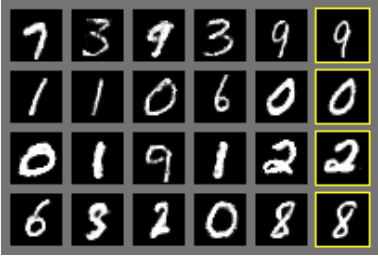
\includegraphics[scale=0.4]{chapter_14/files/gan_mnist.png}
  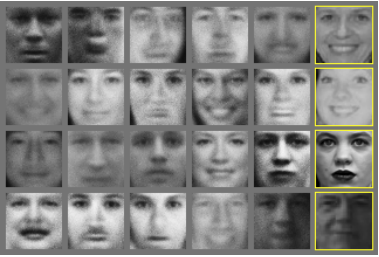
\includegraphics[scale=0.4]{chapter_14/files/gan_faces.png}
  \caption{Generated images from the original GAN paper \cite{goodfellow2014generative}, using images from the MNIST and TFD datasets}
\end{figure}

In 2015, Radford et al\cite{radford2015unsupervised} adapted the then-state-of-the-art convolution neural networks to the GAN framework, creating what they called Deep Convolutional Generative Adversarial Networks (DCGAN). Using deeper convolutional neural networks for both the discriminator and the generators, this extensions of GANs was able to create much more realistic generated images, as seen below. The GAN images are trained on the CIFAR10 dataset, and as is visible, the generated images are not particularly clear (the yellow images show samples from the original data set). On the other hand, when trained on the LSUN dataset of images of bedrooms, DCGAN is able to produce images that are recognizably bedrooms as well.

\begin{figure}[h]
\centering
  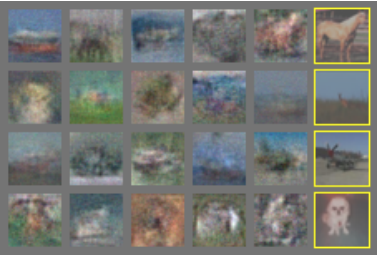
\includegraphics[scale=0.4]{chapter_14/files/gan_images.png}
  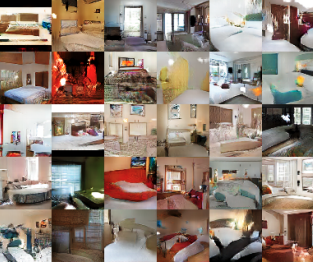
\includegraphics[scale=0.4]{chapter_14/files/dcgan_bedrooms.png}
  \caption{Generated images from the original GAN paper \cite{goodfellow2014generative} (left) vs generated images using DCGAN (right)\cite{radford2015unsupervised}}
\end{figure}